\chapter{Attack Simulation}
\label{cap:attacksimulations}

% point out comparison better! check whole chapter

% old: The combined reliability based \ac{CMA-ES} is the only attack, which is claimed to have a linear increasing complexity for successful attacks on \xpufs that grow linear in their number of used \apufs, as explained in Sec. \ref{sec:essentialattacks} \cite{Becker2015ThePUFs}.
The combined reliability based \ac{CMA-ES} is the only attack, which is claimed to have a linear increasing complexity for successful attacks on \xpufs of arbitrary size, as indicated in Sec. \ref{sec:essentialattacks} \cite{Becker2015ThePUFs}.
Successfully attacked here means to build a model that can predict $80\ \%$ of the challenges from a test set, which contains randomly chosen challenges, correct.
The implementation details of the \ac{CMA-ES} attack and the \apuf, which is basis for the simulations of the \mpuf, is explained in Chap. \ref{cap:simulationdesign}.

This section presents the results of the simulations to verify the success of the \ac{CMA-ES} attack on large \xpufs.
First, the dependency between the number of vote used for \ac{MV} and the number of collected unreliable challenges is examined, as the attack is based on the unreliability of challenges.
% old: After that, the success of the normal reliability based \ac{CMA-ES} attack on \mpufs in comparison to \apufs is evaluated, since they are used to build the \mxpuf.
The normal reliability based \ac{CMA-ES} attack is part of the combined attack on \mxpufs and attacks the underlying \mpufs.
Hence, in the simulation the success of this normal reliability based \ac{CMA-ES} attack on \mpufs in comparison to \apufs is evaluated, since they are used to build the \mxpuf.
Finally, the \ac{CMA-ES} attack is applied to \xpufs and \mxpufs of different size to study whether \ac{MV} can prevent the attack through enabling large \mxpufs. 

% same configuration as for stability simulation, repeat and ref
% ref to machine learning design
%========================================

\section{Detection of Unreliable Challenges}
\label{sec:detectionofunreliablechallenges}

For the reliability based \ac{CMA-ES} attack on \apufs it is crucial to find challenges, which evaluate differently at multiple evaluations, as termed in Sec. \ref{sec:reliability}.
To find these challenges and their reliability $\gls{h}$ every challenge $\gls{c}$ of a set will be evaluated $\gls{j}$ times.
Consequently, the reliability $\gls{h}$ will be computed for every challenge by Eq. (\ref{equ:reliability}).
% old: Do not get confused with the notions stability and reliability as the definition of reliability differs for the \ac{CMA-ES} attack, as explained in Sec. \ref{sec:reliability}.
Note that the notions of stability and reliability are slightly different for the \ac{CMA-ES} attack, as defined in Sec. \ref{sec:reliability}.

When using \ac{MV} to increase the stability of the \apuf, finding challenges with lower reliability becomes more difficult.
Accordingly, Fig. \ref{fig:cmamajorityvotemeasurementrelation} shows the relation between the increase of votes $\gls{m}$ and the decrease of found challenges with lowered reliability $\gls{h}$.
%old: In this case, a lowered reliability is already reached if a challenge $\gls{c}$ evaluates one or multiple times different to the rest of the evaluations for $\gls{j}$ evaluations and is called unreliable. 
In this case, a lowered reliability is already reached if a challenge $\gls{c}$ evaluates one or multiple times different to the rest of the $\gls{j}$ evaluations and is thus called unreliable.
There are four line graphs for the different numbers of evaluations $\gls{j}$.

\begin{figure}[ht]
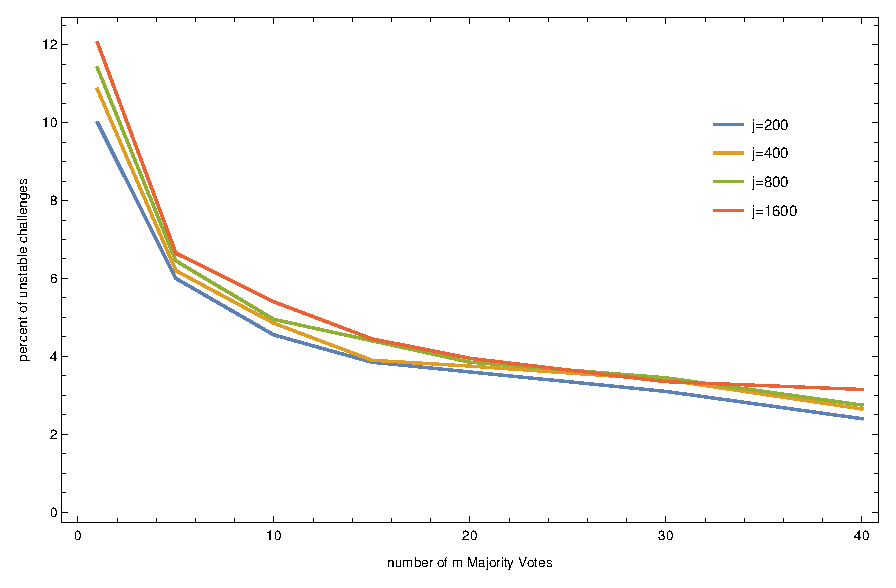
\includegraphics[width=1.00\textwidth]{images/mv-measurements-unstableChallenges.eps}
% \noindent\includegraphics[width=1.00\textwidth, height=3cm, draft]{example-image-a}
\caption[Proportion of unreliable challenges]{Proportion of unreliable challenges for different values of $\gls{m}$ \acp{MV}. The different line graphs represent the number of evaluations $\gls{j}$ in $200, 400, 800, 1600$. The slight distance between the graphs in the beginning shows the very little increase of found unreliable challenges with increasing number of evaluations $\gls{j}$ and how this gap resolves with introducing of \ac{MV}.}
\label{fig:cmamajorityvotemeasurementrelation}
\end{figure}

% Old and wrong: The raising gradient of all four graphs could lead to the same assumption display the subsiding impact of \ac{MV} with rising $\gls{m}$ as explained in Sec. \ref{sec:stabilityimprovementbymajorityvote}.
The raising gradient of all four graphs could lead to the same assumption of the subsiding impact of \ac{MV} with rising $\gls{m}$, as mentioned in Sec. \ref{sec:stabilityimprovementbymajorityvote}.
However, the linear course of the graph, showed by the logarithmic Fig. \ref{fig:cmamajorityvotemeasurementrelationloglog}, suggest that this is not the case and supports the result of Sec. \ref{sec:stabilityimprovementbymajorityvote}.

\begin{figure}[ht]
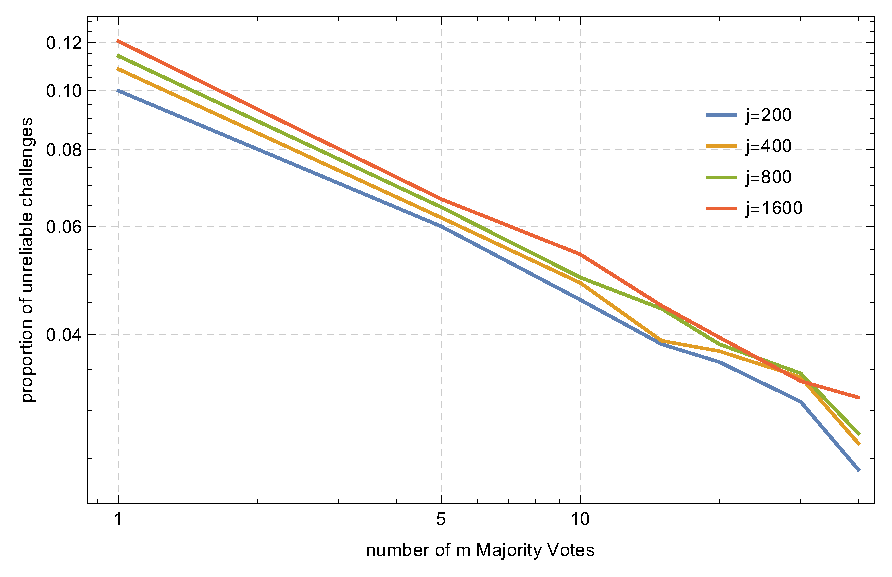
\includegraphics[width=1.00\textwidth]{images/mv-measurements-unstableChallenges_loglog.eps}
% \noindent\includegraphics[width=1.00\textwidth, height=3cm, draft]{example-image-a}
\caption[Proportion of unreliable challenges logarithmic]{The line graphs show the proportions of unreliable challenges for different values of $\gls{m}$ \acp{MV} similar to Fig. \ref{fig:cmamajorityvotemeasurementrelation} yet in logarithmic scale. The linear course of the graphs suggest that there is no decline of the stability improving impact of \ac{MV} with increasing $\gls{m}$ used for \mpufs.}
\label{fig:cmamajorityvotemeasurementrelationloglog}
\end{figure}

The slight difference between the graphs in both figures shows that increasing the number of evaluation $\gls{j}$ does not necessarily provides more challenges with lowered reliability $\gls{h}$.
Without \ac{MV} there is a little increase of found challenges with lowered reliability $\gls{h}$.
Though, with applying \ac{MV} this increase disappears with growing $\gls{m}$.

The results presented in this section verify that the number of unreliable challenges decreases with an increase of used \ac{MV} votes.
Despite the use of \ac{MV}, unreliable challenges are occurring.

%========================================

\section{\apufs vs. \mpufs}
\label{sec:arbitervsmajorityarbiter}

This section describes the results of the simulation used to scrutinize the success of the \ac{CMA-ES} attacks, presented in Sec. \ref{sec:cma-esdesign}, on \mpufs in comparison to \apufs.
Through the comparison with the success of the attack on \apuf the impact of \ac{MV} can be evaluated.

The \apuf used for the simulation has $\gls{n} = 32$ stages.
For the attack a training set of $10000$ \acp{CRP} and a number of evaluation times of $\gls{j} = 100$ were used.
Since the \ac{CMA-ES} attack not always approximates to a model, which performs well on the challenges of the test set, it has to be restarted.
The number of needed starts of the attack till a desired model has been approximated is called number of attack executions.

A model produced by the attack is defined to perform well if it evaluates $80\ \%$ of the $10000$ \acp{CRP} of the test set correct.
Both test set and training set are independent randomly chosen sets of challenges $\gls{c}$.
% The exit criteria sigma of the \ac{CMA-ES} attack as explained in Sec. \ref{sec:cma-esdesign} is set to $0.2$ and stops the attack despite if the attack approximates to a model, which performs well on the test set or not.
The minimum step-size sigma, used in the attack as termination criteria, explained in Sec. \ref{sec:cma-esdesign}, is set to the value $0.2$.
Reaching this limit stops the attack regardless if a well performing model is approximated or not.

For a growing number of \ac{MV} $\gls{m}$ there is an increase of needed executions of the attack to approximate to a model, which performs well on the test set, as shown in Fig \ref{fig:cmasingleattackcorrelation}.
The growing gradient of the graph shows the growing exponential increase of needed attack executions to gain well performing models.
From $\gls{m} = 80$ \acp{MV} on the gradient of the graph is greater than $1$.
Hence, the slope of the number of attack executions is greater than the polynomial degree $1$.

\begin{figure}[ht]
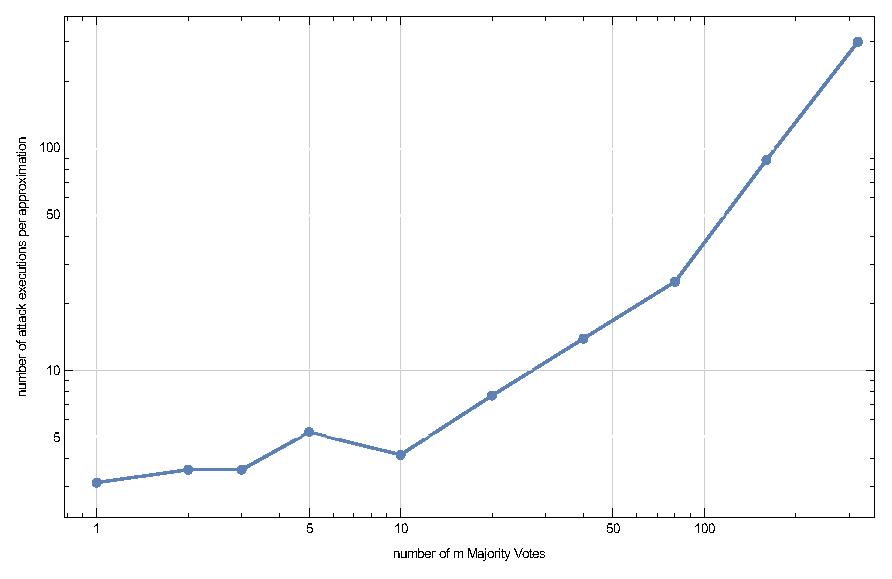
\includegraphics[width=1.00\textwidth]{images/single-mv-classification-cma-attack-correlation.eps}
% \noindent\includegraphics[width=1.00\textwidth, height=3cm, draft]{example-image-a}
\caption[Needed \acs{CMA-ES} attack executions for \mpufs]{Number of attack executions per approximation to a well performing model. A well performing model evaluates $80\ \%$ of the $10000$ test set \acp{CRP} correct. The rising gradient of the graph shows the growing exponential increase of the number of attack executions.}
\label{fig:cmasingleattackcorrelation}
\end{figure}

Apart from the increasing number of attack executions the performance of the computed models decreases with the growth of $\gls{m}$, as shown in Fig. \ref{fig:cmasingleattackcorrectness}.
The graph displays how the proportion of correct evaluated challenges $\gls{c}$ of the test set lowers linear with a linear rise of the number of \ac{MV} $\gls{m}$.
This indirect correlation implies that with growing number of \ac{MV} $\gls{m}$ the proportion of the correct evaluated challenges $\gls{c}$ of the test set decreases for well performing models build by the \ac{CMA-ES} attack.
The values of both Fig. \ref{fig:cmasingleattackcorrelation} and Fig. \ref{fig:cmasingleattackcorrectness} are average values of minimum $10$ well performing models.

\begin{figure}[ht]
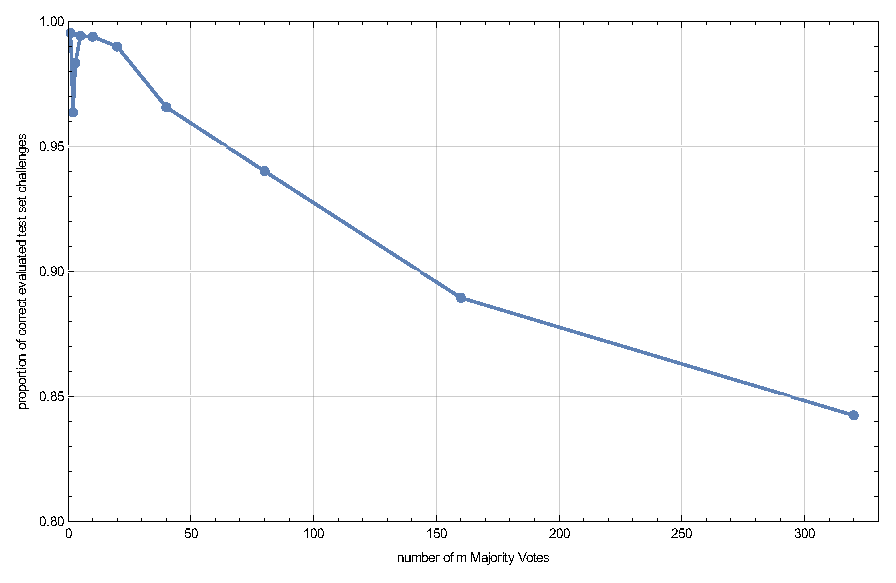
\includegraphics[width=1.00\textwidth]{images/single-mv-classification-cma-attack-correctness.eps}
% \noindent\includegraphics[width=1.00\textwidth, height=3cm, draft]{example-image-a}
\caption[Proportion of correct evaluated test set challenges for Arbiter \puf models and Majority Arbiter \puf models]{Proportion of correct evaluated test set \acp{CRP} of a well performing model build by a \ac{CMA-ES} attack. The linear decrease of the graph shows the decrease of the proportion of correct evaluated challenges $\gls{c}$ by a well performing model. The values used are average values of minimum $10$ well performing model or at least $2000$ attack executions.}
\label{fig:cmasingleattackcorrectness}
\end{figure}

% The results of this section show that with a growing number of votes $\gls{m}$ the required number of \ac{CMA-ES} attack executions increases greatly as well.
The results of this section show that the required number of \ac{CMA-ES} attack executions increases faster than the growing number of votes $\gls{m}$ from a certain point on.
Applying a large number of votes can be used to minimize the likelihood of a successful attack.
\ac{MV} improves the ability of \apufs to resist reliability based \ac{CMA-ES} attacks.

%========================================

\section{\acs{XOR} \apufs vs. Majority \acs{XOR} \apufs}
\label{sec:xorarbitervsmajorityxorarbiter}

% \xpuf to unstable with growing k

This section presents the results of the simulation to verify the success of the combined \ac{CMA-ES} attacks, as introduced in Sec. \ref{sec:attackcombination}, on \mxpufs in comparison to \xpufs.
Through the comparison with the success of the attack on \xpuf the impact of \ac{MV} can be evaluated.
First, the results of the attack on \xpufs are compared with the results of the attack on \mxpufs.
Subsequently, limits of the attack on \mxpufs are outlined.
Finally, the modifications of the preconditions for the attack and the according results are shown.

To gain comparable results the simulation uses the same preconditions for the attacks on \xpufs and \mxpufs.
All \pufs in this simulation have $n = 32$ stages.
The number of challenges in the training set increases linear with the growth of the number of $k$ \apufs or $k$ \mpufs.
The simulations starts with $5000$ training set challenges for $k = 2$ and doubles the number of training set challenges for the double number of $k$.
All training set challenges are individually randomly chosen for all attacks.

A test set is used to evaluate the performance of the learned model.
The attack is successful when the learned model evaluates $80\ \%$ of the test set challenges correct and thus is defined to perform well.
The test set contains $2000$ individually randomly chosen challenges for all measurements, since only the complexity of the attack grows for a similar results.
The number of $5000$ training set challenges in combination with $2000$ test set challenges were chosen for the reason that attacks on \xpufs with $k = 2$ and $k = 4$ with accordingly $10000$ training set challenges were able to build well performing models.

\todo{update values}
\begin{figure}[ht]
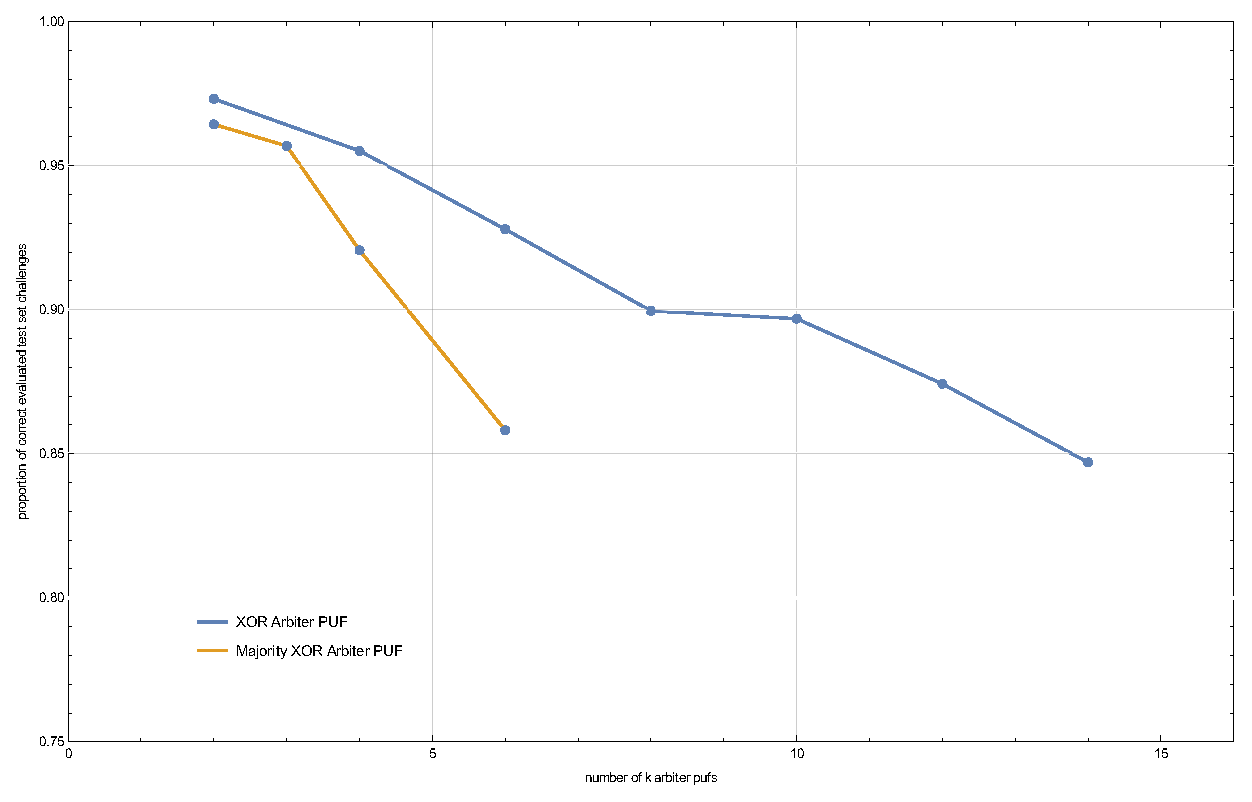
\includegraphics[width=1.00\textwidth]{images/xor-cma-attack-performance.eps}
% \noindent\includegraphics[width=1.00\textwidth, height=3cm, draft]{example-image-a}
\caption[Proportion of correct evaluated test set challenges for \acs{XOR} Arbiter \puf models and Majority \acs{XOR} Arbiter \puf models]{Proportion of correct evaluated test set challenges of \xpuf models and \mxpuf models. All values are average values of 10 independent attacks. The number of used training set challenges and votes $\gls{m}$ is chosen according to the Tab. \ref{tab:cmamultinumbervotes}. The test set contains for all attack $2000$ challenges.}
\label{fig:cmamultiattackmodelperformance}
\end{figure}

Fig. \ref{fig:cmamultiattackmodelperformance} shows the proportion of correct evaluated test set challenges by well performing models produced by the attacks for $2 \le \gls{k} \le 12$.
Every value is the average of $10$ successfully learned models.
Since the attack is not deterministic, only attack executions that approximate well performing models are counted.
% wrong: There are no significant differences in the needed number of attack executions for different numbers of $\gls{k}$ neither for \xpufs nor for \mxpufs.
The number of required attack executions for a successful attack are similar for all attacks on \xpufs.
\todo{rose significant: be more specific!}
In the case of \mxpufs the number of attack executions needed to obtain a well performing model rose significant for $k = 4$ and $k = 6$.

The numbers of \ac{MV} votes $\gls{m}$ used for the \mxpufs in Fig. \ref{fig:cmamultiattackmodelperformance} are determined by the results of the simulations in Sec. \ref{sec:majorityvotegrowth}.
This simulations approximated the required numbers of votes to gain stable large \mxpufs, which means to reach $\Pr[\protect\Stab(\gls{c}) \ge 95\ \%] \ge 95\ \%$, for different $\gls{k}$.
In Tab. \ref{tab:cmamultinumbervotes} the used values $\gls{m}$ for different values of $\gls{k}$ and the number of training set challenges that are similar to \xpufs and \mxpufs are displayed.

\todo{update values + values in text!}
\begin{table}[ht]
\centering
\begin{tabular}{|l|c|c|c|c|c|c|c|}
\hline
number of $\gls{k}$ & 2 & 3 & 4 & 6 & 8 & 10 & 12\\
\hline
number of training set challenges ($\cdot 10^3$) & 5 & 7.5 & 10 & 15 & 20 & 25 & 30\\
% number of training set challenges & $5*10^3$ & $7.5 \cdot 10^3$ & $10 \cdot 10^3$ & $15 \cdot 10^3$ & $20 \cdot 10^3$ & $25 \cdot 10^3$ & $30 \cdot 10^3$\\
\hline
number of votes $\gls{m}$ & 5 & 9 & 17 & 29 & 64 & 100 & 150\\
\hline
\end{tabular}
\caption[Number of votes and challenges used for \acs{CMA-ES} attack]{Number of used training set challenges for the attack on \xpufs and \mxpufs. Number of \ac{MV} votes used for the according \mxpufs determined by the simulation in Sec. \ref{sec:majorityvotegrowth}.}
\label{tab:cmamultinumbervotes}
\end{table}

The Fig. \ref{fig:cmamultiattackmodelperformance} states the decrease of the performance of models, which are approximated of \xpufs.
With this decrease in performance a continuous trend would already lead to not well performing models learned by an attack on large \xpufs.
The attack would not be successful for large \xpufs, if it was possible to build them stable.
If there was no impact of \ac{MV} on the attack success, the models, approximated by the attack on \mxpufs, would reach the same performance.
For the case that the attack benefits of \ac{MV}, the performance values of the attack on \xpufs would be exceeded.
However, the line graph for well performing models of the attack on \mxpufs stops after $k = 6$.
The attack was not able to learn well performing models of \mxpufs that have a $\gls{k} \ge 8$ and uses $\gls{m}$ votes and the number of challenges, as defined in Tab. \ref{tab:cmamultinumbervotes}.
% how many attack executions to prove this

Nevertheless, the attack could be successful and train models, which fulfill a certain performance, with a polynomial increase in the number of used training set challenges.
To study the success of the attack on \mxpufs, we approximate the required training set \acp{CRP} for successful attacks that lead to models with a given performance by binary search.
In Fig. \ref{fig:cmamultiattackrequiredcrp} a comparison between the required training set challenges of the attack on \xpufs and \mxpufs is shown.
The raising gradient of the graph states the exponential increase in demanded \acp{CRP} for a successful attack on \mxpufs that use the according number of votes $\gls{m}$, as display in Tab. \ref{tab:cmamultinumbervotes}.

\todo{update values}
\begin{figure}[ht]
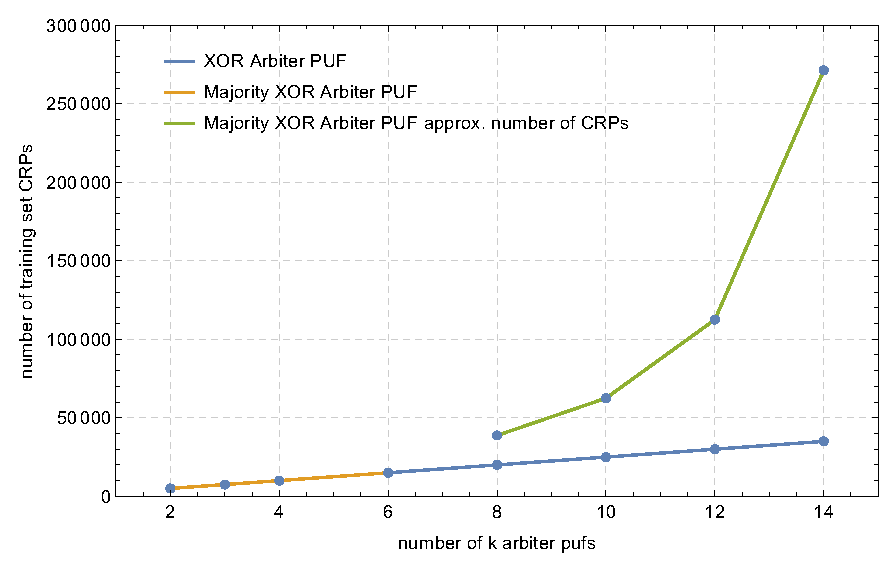
\includegraphics[width=1.00\textwidth]{images/xor-cma-attack-crps.eps}
% \noindent\includegraphics[width=1.00\textwidth, height=3cm, draft]{example-image-a}
\caption[Number of used training set challenges]{Number of used training set challenges to attack different \pufs. The necessary number of training set challenges for well performing model with a continuous performance are approximated by binary search.}
\label{fig:cmamultiattackrequiredcrp}
\end{figure}

To scrutinize the approximated required number of \acp{CRP}, $10$ successful attacks are performed for every $k$ and the average proportion of correct evaluated test set challenges by well performing models are compared with the results of the attacks on \xpufs in Fig. \ref{fig:cmamultiattackmvmodelperformance}.
%wrong: The similarity of the graphs on the attack on \xpufs and \mxpufs with the approximated required number of training challenges verifies that the attack results in the similar well performing model by a exponential increase of training challenges.
The continuous high performance of the models, which are learned with the approximated number of training set challenges, shows that the large increase of required challenge in Fig. \ref{fig:cmamultiattackrequiredcrp} are needed to obtain well performing models of the attacks.
This is important, since otherwise with a growing number $\gls{k}$ the performance of the models would subside and the attack would not be successful.

\todo{update values}
\begin{figure}[ht]
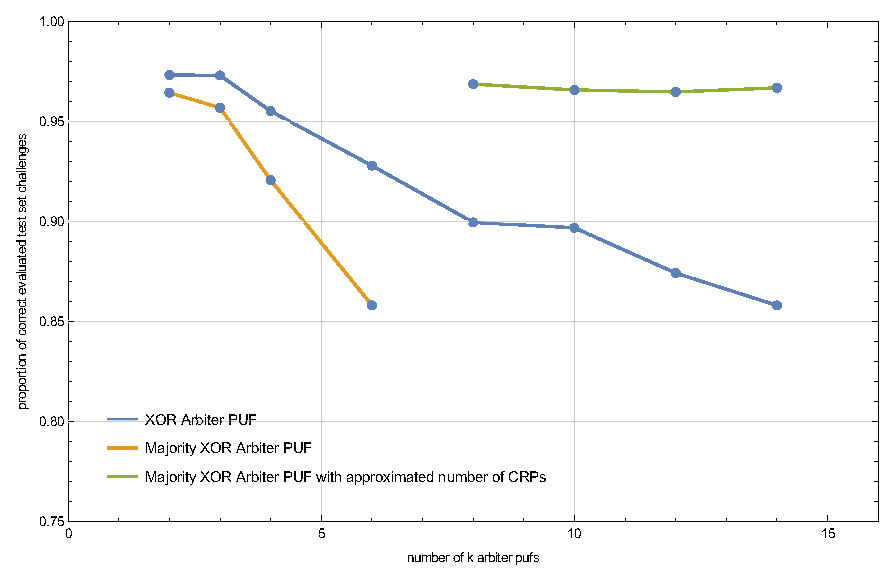
\includegraphics[width=1.00\textwidth]{images/xor-cma-attack-approx.eps}
% \noindent\includegraphics[width=1.00\textwidth, height=3cm, draft]{example-image-a}
\caption[Proportion of correct evaluated test set challenges for Majority \acs{XOR} \puf models with approximated required number of training set challenges]{Proportion of correct evaluated test set challenges of well performing models trained with an approximated number of training set challenges. To measure the performance of the model a test set with $2000$ \acp{CRP} is used and the results are compared with the results of the attack simulations of Fig. \ref{fig:cmamultiattackmodelperformance}. The number of used training set challenges is displayed by Fig. \ref{fig:cmamultiattackrequiredcrp}.}
\label{fig:cmamultiattackmvmodelperformance}
\end{figure}

% The exponential raise of the required number of training set challenges for a  the same attack results confirms the impact of \ac{MV} on the combined \ac{CMA-ES} attack.
The exponential raise of the required number of training set challenges for successful attacks confirms the impact of \ac{MV} on the combined \ac{CMA-ES} attack.
The complexity of the attack grows exponentially, since the number of needed challenges to train the model increases exponentially for \mxpufs with a linear growth of the number of \mpufs.

The claim, which states that the complexity of the combined \ac{CMA-ES} attack grows linear for \xpufs with linear growth in $\gls{k}$, is not directly refuted.
However, the performance of the learned model subsides and thus the attack will not be able to learn models with a certain performance for a large given number of $\gls{k}$.

Nevertheless, Chap. \ref{cap:stabilitysimulation} outlined that it is possible to build large \xpufs with the principle of \ac{MV} called \mxpufs.
In Sec. \ref{sec:essentialattacks} we state that only the combined \ac{CMA-ES} attack is relevant to large \xpufs and thus \mxpufs.
As a result, large \mxpufs can not be successfully modeled by the combined \ac{CMA-ES} attack or any other currently known attack.

% maybe: why low number of crps -> impact not measurable with high number as boundary will be not reached
% abgrenzung von normal CMA-ES (könnte einfach alle werte auf einmal lernen), jedoch nur relevant fuer kleine k
%========================================

